\documentclass[12pt, letterpaper]{../assignment}
\usepackage{graphicx}
\usepackage{courier}
\usepackage{minted}
\usepackage{amsmath}
\usepackage{commath}
\usepackage{amssymb}
\usepackage{amsfonts} 
\usepackage{cancel}
\usepackage{enumitem}
\usepackage{array}

\usepackage{tikz}
\usetikzlibrary{shapes,arrows,positioning}

\usemintedstyle{monokai}
\oddsidemargin = 0pt
\exercisesheet{Module 11}{Practice Assignment}
\student{Austin Barrilleaux}
\courselabel{EN 525.609}
\semester{Fall 2023}
\usepackage[backend=bibtex,style=numeric,sorting=none]{biblatex}
\bibliography{reference}
\usepackage{color}
\definecolor{light-gray}{rgb}{0.2,0.2,0.2}
\setminted{bgcolor=light-gray}
\setlength{\parindent}{0pt}

\makeatletter
\patchcmd{\minted@colorbg}{\noindent}{\medskip\noindent}{}{}
\apptocmd{\endminted@colorbg}{\par\medskip}{}{}
\makeatother

\begin{document}
\subsection*{Problem 1}
% \subsubsection*{Solve the following practice problems in the 9th edition textbook.\\
% \begin{itemize}
%     \item Chapter 8:
%     \begin{itemize}
%         \item 8-1
%         \item 8-5
%     \end{itemize}
% \end{itemize}}

\subsubsection*{Do the following homework problems from the text book:\\
\begin{itemize}
    \item 8-39 (a)
\end{itemize}}

\subsubsection*{8-39. 
The forward-path transfer functions of unity-feedback control systems are given in the following equations.
Plot the Bode diagram of $\mathbf{G(j\omega) / K}$, and do the following:\\
(1) Find the value of $K$ so that the gain margin of the system is $\mathbf{20}$ dB.\\
(2) Find the value of $K$ so that the phase margin of the system is $\mathbf{45^\circ}$.}

\subsubsection*{(a) \ \ \ $\mathbf{ \dfrac{K}{s(1 + 0.1 s)( 1 + 0.5 s )}}$}

We can plot the Bode diagram using the \texttt{margin()} function in MATLAB, when $K = 1$.
Evaluating $\texttt{\text{margin}(1/(s*(1 + 0.1*s)*(1 + 0.5*s)))}$ generates the following plot:

\begin{figure}[H]
    \centering
    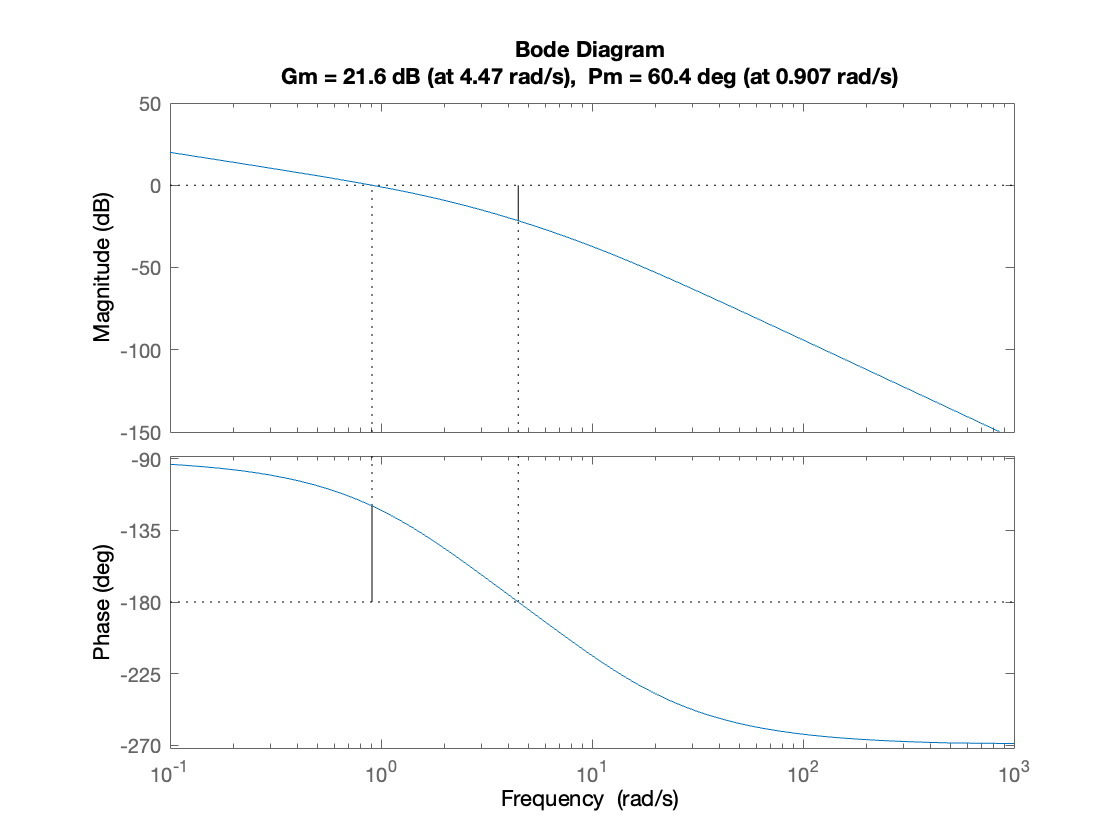
\includegraphics[width=1\linewidth]{./figures/BodePlot_K_1.png}
    \caption{Bode Plot: K = 1}
 \end{figure}

The transfer function in question can be written as:

$$ G(j\omega) = \frac{K}{- 0.05 j \omega ^3 - 0.6 \omega ^2 + j \omega }
              = \frac{K}{- 0.6 \omega ^2 - j(0.05\omega ^3 - \omega) }$$

The magnitude of $G(j\omega)$, is calculated as:

$$ |G(j\omega)| = \frac{|K|}{|- 0.05 j \omega ^3 - 0.6 \omega ^2 + j \omega |}
                = \frac{K}{\sqrt{0.0025 \omega^6 + 0.26 \omega^4 + \omega^2 }}$$

Setting the magnitude of the gain equal to 1, we can solve for the gain crossover frequency.
For this we will solve initially with $K=1$:

$$ 1 = \frac{1}{\sqrt{0.0025 \omega_g^6 + 0.26 \omega_g^4 + \omega_g^2 }}$$

This becomes:

$$ 0.0025 \omega_g^6 + 0.26 \omega_g^4 + \omega_g^2 - 1^2  = 0 $$

Solving for the roots of this equation, using the MATLAB $\texttt{roots()}$ function:


$$ \texttt{roots}([0.0025,0,0.26,0,1,0,-1]) = \left[\begin{array}{rr} 
    0.0000 &+ j9.9979\\
    0.0000 &- j9.9979\\
    0.0000 &+ j2.2055\\
    0.0000 &- j2.2055\\
   -0.9070 & \\
   \mathbf{ 0.9070} & \\
    \end{array} \right]\ $$

The gain crossover frequency is $ \omega_g = 0.9070 \ \text{rad/s} $.
\\\\
Taking the initial transfer function, we can rewrite it as:

\begin{equation*}
\begin{aligned}
G(j\omega) &= \frac{K}{- 0.6 \omega ^2 - j(0.05\omega ^3 - \omega) }
        \left(\frac{- 0.6 \omega ^2 + j(0.05\omega ^3 - \omega)}
                   {- 0.6 \omega ^2 + j(0.05\omega ^3 - \omega)}\right)\\
           & = \frac{K(- 0.6 \omega ^2 + j(0.05\omega ^3 - \omega))}
                    { 0.36 \omega ^4 + (0.05\omega ^3 - \omega)^2 }
\end{aligned}
\end{equation*}

The phase angle for this equation is:

$$ \angle G(j\omega) = \tan^{-1} \left( \frac{0.05\omega ^3 - \omega}{- 0.6 \omega ^2} \right)
                     = \tan^{-1} \left( \frac{0.05\omega ^2 - 1}{- 0.6 \omega} \right) $$

We can determine the phase crossover frequency as:

$$ \text{Im}\{G(j\omega)\} = 0.05\omega_p ^2 - 1 = 0$$

Which solves for $\omega_p$ as:

$$ \omega_p = \sqrt{20} = 4.4721 $$

The phase crossover frequency is $ \omega_p =  4.4721 \ \text{rad/s} $.
\\\\
The gain margin can be calculated as:

$$ |G(j\omega_p)| = 10/120 $$

$$ -20 \log_{10} (10/120) = -21.5836 \ \text{dB} $$

If we want to make the gain margin 20 dB, we have to increase the gain magnitude at phase crossover frequency from $-21.5836$ to $-20$,
which is an increase of $1.5836$ dB.
We can calculate this gain factor as:

$$ K = 10^{(1.5836/20)} = 1.2 $$

\begin{answer}
The value of $K$ so that the gain margin of the system is $\mathbf{20}$ dB, is $K = 1.2$.
\end{answer}

We can confirm this using the \texttt{margin()} function in MATLAB.
Evaluating \\ $\texttt{\text{margin}(1.2/(s*(1 + 0.1*s)*(1 + 0.5*s)))}$ generates the following plot:

\begin{figure}[H]
    \centering
    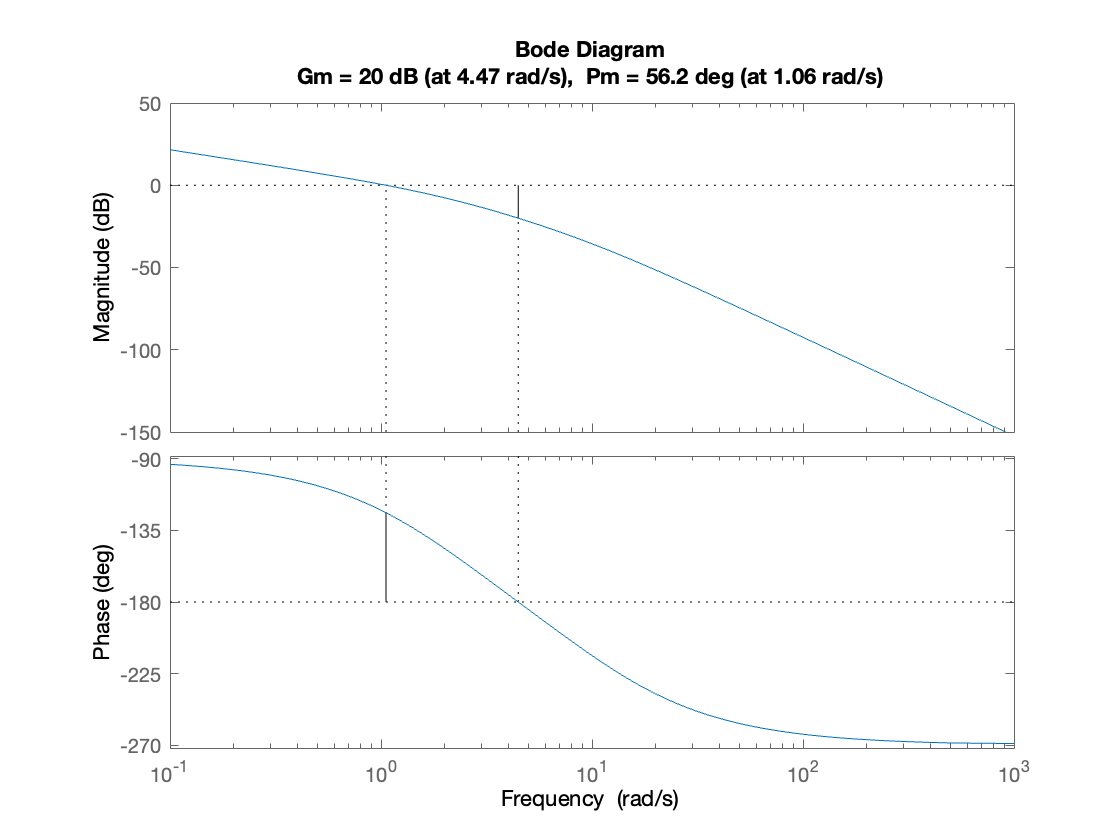
\includegraphics[width=1\linewidth]{./figures/BodePlot_K_1.2.png}
    \caption{Bode Plot: K = 1.2}
 \end{figure}

We can see that the gain margin is indeed 20 dB. 
\\\\
We can solve for the phase margin as:

$$ \angle G(j\omega_g) = \tan^{-1} \left( \frac{0.05\omega_g ^2 - 1}{- 0.6 \omega_g} \right) $$

$$ \angle G(j0.907) = \tan^{-1} \left( \frac{0.05(0.907) ^2 - 1}{- 0.6 (0.907)} \right) = 60.4231^\circ $$

If we want to make the phase margin equal to $45^\circ$,
we need to set the phase angle equation equal to $45^\circ$, to solve for the frequency at which the phase angle is equal to $45^\circ$.
We can write this as:

$$ \angle G(j\omega_g) = 45^\circ = \tan^{-1} \left( \frac{0.05\omega_g ^2 - 1}{- 0.6 \omega_g} \right) $$

This can be rewritten as:

$$ \tan(45^\circ) = 1 =\left( \frac{0.05\omega_{45^\circ} ^2 - 1}{- 0.6 \omega_{45^\circ}} \right) $$

Further:

$$ 0.05\omega_{45^\circ} ^2 + 0.6 \omega_{45^\circ} - 1 $$

Solving for the roots of this equation, using the MATLAB $\texttt{roots()}$ function:

$$ \texttt{roots}([0.05,0.6,-1]) = \left[\begin{array}{r} 
    -13.4833\\
    \mathbf{1.4833}
    \end{array} \right]\ $$

The frequency at which the phase angle is equal to $45^\circ$, is 1.4833 rad/s.
\\
If we want this to be the gain crossover frequency, we need to set the magnitude equal to 1,
where $\omega = 1.4833 $:

$$ 1 = \frac{K}{\sqrt{0.0025 (1.4833)^6 + 0.26 (1.4833)^4 + (1.4833)^2 }}$$

\begin{answer}
Solving this, $K = 1.8669$ gives us a phase angle of $45^\circ$.
\end{answer}

We can confirm this using the \texttt{margin()} function in MATLAB.
Evaluating \\ $\texttt{\text{margin}(1.8669/(s*(1 + 0.1*s)*(1 + 0.5*s)))}$ generates the following plot:

\begin{figure}[H]
    \centering
    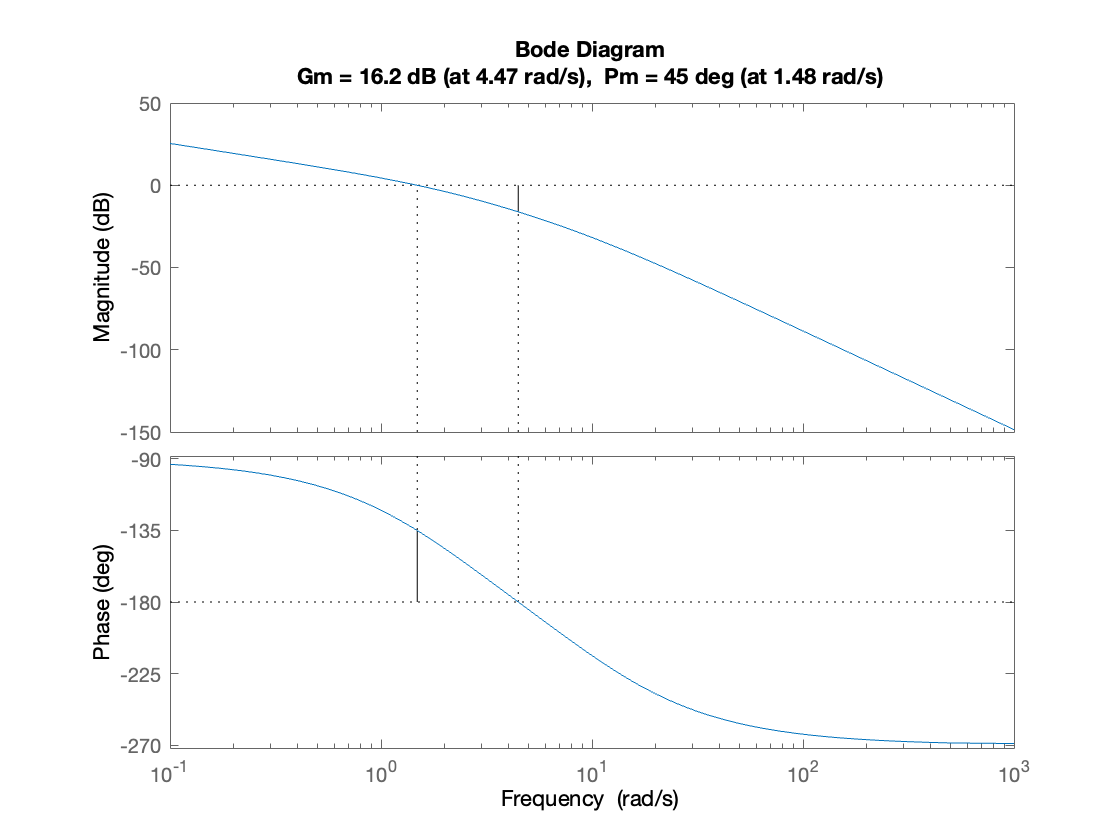
\includegraphics[width=1\linewidth]{./figures/BodePlot_K_1.8669.png}
    \caption{Bode Plot: K = 1.8669}
\end{figure}

We can see that the phase margin is indeed $45^\circ$. 

\subsection*{Problem 2}
\subsubsection*{Consider the following feedback system:}
\begin{figure}[H]
    \centering
    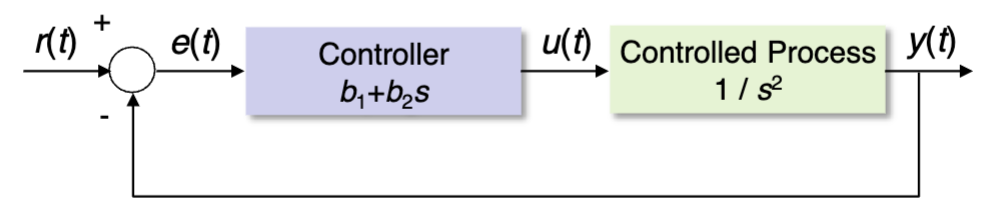
\includegraphics[width=0.7\linewidth]{./figures/Q2_Block_Diagram.png}
    \caption{Feedback System}
\end{figure}

\subsubsection*{
(a) Compute the sensitivity function, $\mathbf{S^T_G (s)}$,
and the complementary sensitivity function, $\mathbf{T(s)}$.}

For this system:

$$ D(s)G(s) = \frac{b_1 + b_2 s}{s^2} $$

The sensitivity function is:

\begin{answer}
    $$ S^T_G (s) =  [1 + D(s)G(s)]^{-1} = \frac{s^2}{b_1 + b_2 s + s^2} $$
\end{answer}

The complimentary sensitivity function is the closed-loop transfer function. Therefor:

\begin{answer}
    $$ T(s) =  \frac{D(s)G(s)}{1 + D(s)G(s)} = \frac{b_1 + b_2 s}{b_1 + b_2 s + s^2} $$
\end{answer}
\subsubsection*{
(b) Assume a critically damped system ($\mathbf{\zeta=1}$) and a (normalized) natural frequency $\mathbf{\omega_n=1}$.
Using MATLAB, plot the magnitude response of the sensitivity and complimentary sensitivity functions $\mathbf{S(s)}$ and $\mathbf{T(s)}$ on the same plot.
At what frequency does $\mathbf{S(s)=T(s)}$? What can be said about the roles of $\mathbf{S(s)}$ and $\mathbf{T(s)}$ at this frequency?}

Assuming a critically damped system ($\zeta=1$) and a (normalized) natural frequency $\omega_n=1$,
for this system:

$$ b_1 = \omega_n^2 = 1^2 \ \ \rightarrow \ \ b_1 = 1 $$

$$ 2 \zeta \omega_n s = b_2 s  \ \ \rightarrow \ \ b_2 = 2 \zeta \omega_n = 2 (1) (1) = 2 $$

The sensitivity function is:

$$ S(s) = \frac{s^2}{1 + 2 s + s^2} $$

The complimentary sensitivity function is:

$$ T(s) = \frac{1 + 2 s}{1 + 2 s + s^2} $$

Plotting both of these in MATLAB:
\begin{figure}[H]
    \centering
    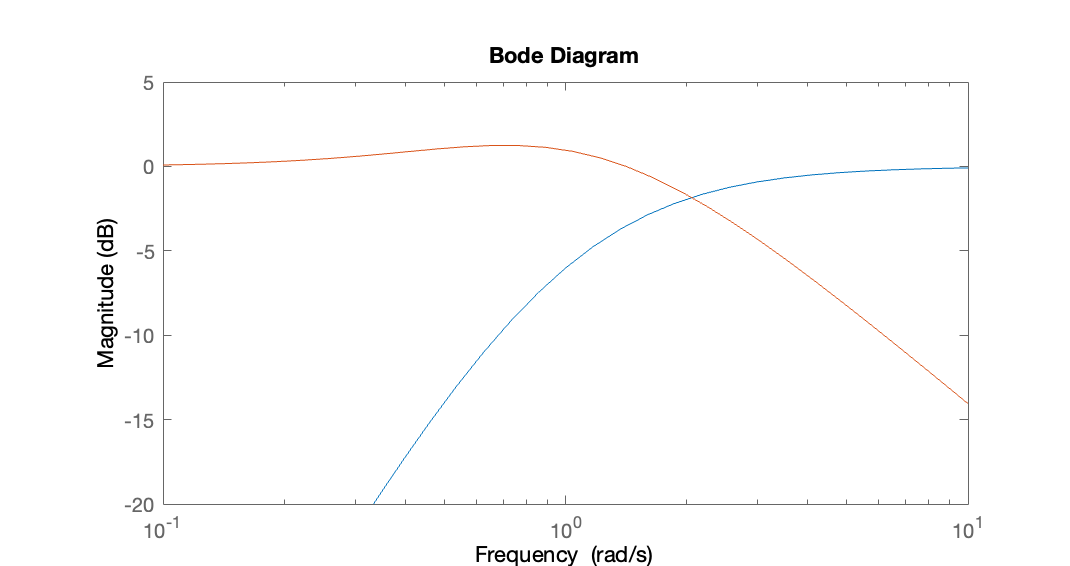
\includegraphics[width=1\linewidth]{./figures/Q2_Bode_Mag.png}
    \caption{Sensitivity \& Complementary Sensitivity}
\end{figure}

\begin{answer}
The frequency when $S(s) = T(s)$ is, $\omega = 2.05887 \ \text{rad/s}$.
\end{answer}

\begin{answer} \textbf{
When designing a system there are two desires,
good tracking and disturbance rejection which is occurs when $S(s)$ is small and $T(s)$ is large,
and good noise rejection when $S(s)$ is large and $T(s)$ is small.
The point at which $S(s) = T(s)$ is the point at which both of those desires share equal priority.
If a larger or smaller frequency is chosen,
then one or the other of those is getting prioritized at the expense of the other.}
\end{answer}

\subsection*{Problem 2}
\subsubsection*{Consider the following (non-min phase) feedback system,
where the CLTF, $\mathbf{T(s)}$, is stable for: $\mathbf{-2<K<1}$}.
\begin{figure}[H]
    \centering
    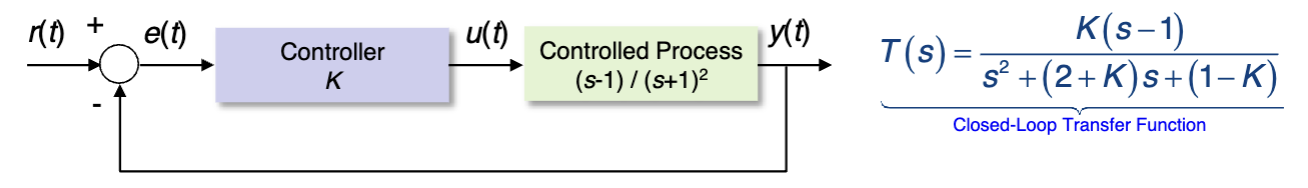
\includegraphics[width=1\linewidth]{./figures/Q3_Block_Diagram.png}
    \caption{ Non-Min Phase Feedback System}
\end{figure}

\subsubsection*{(a) Compute the expression for SSE}

The closed loop transfer function is:

$$ T(s) = \frac{Y(s)}{R(s)} = \frac{K(s-1)}{s^2 + (s+K)s + (1-K)}  $$

The steady state response is:

$$ y_{ss}(t) = \lim_{s \to 0} sY(s) \bigg|_{R(s) = 1/s}
    = s \left(\frac{1}{s}\right)\left[\frac{K(s-1)}{s^2 + (s+K)s + (1-K)}\right]_{s=0} $$

This simplifies to:

$$ y_{ss}(t) = \left[\frac{K(s-1)}{s^2 + (s+K)s + (1-K)}\right]_{s=0}  $$

Evaluating when $s=0$:

$$ y_{ss}(t) = \frac{-K}{1-K} $$

The steady state error is:

\begin{answer}
$$ e_{ss}(t) = r(t) - y_{ss}(t) = 1 - \frac{-K}{1-K} $$
\end{answer}

\subsubsection*{(b) At what (stable) gain is the SSE=0: [$\mathbf{e_{ss}(t) = 0}$]?}

If we set $e_{ss}(t) = 0$, we can solve for the gain:

\begin{answer}
$$ e_{ss}(t) = 0 = 1 - \frac{-K}{1-K}
    \ \ \rightarrow \ \ 1 = \frac{K}{1-K}
    \ \ \rightarrow \ \ K = \frac{1}{2} $$
\end{answer}

\subsubsection*{(c) Using the gain found above,
use MATLAB to plot the system step response to a negative step $\mathbf{R(s)=-1/s}$.
What's unusual about this response?}

We can plot a negative step response using the following MATLAB command:

\color{white}
\begin{minted}{matlab}
    K = 1/2
    T = K * (s-1)/(s^2 + (2 + K)*s + (1-K))
    step(T,stepDataOptions('StepAmplitude',-1))
\end{minted}
\color{black}

It produces this step response:
\begin{figure}[H]
    \centering
    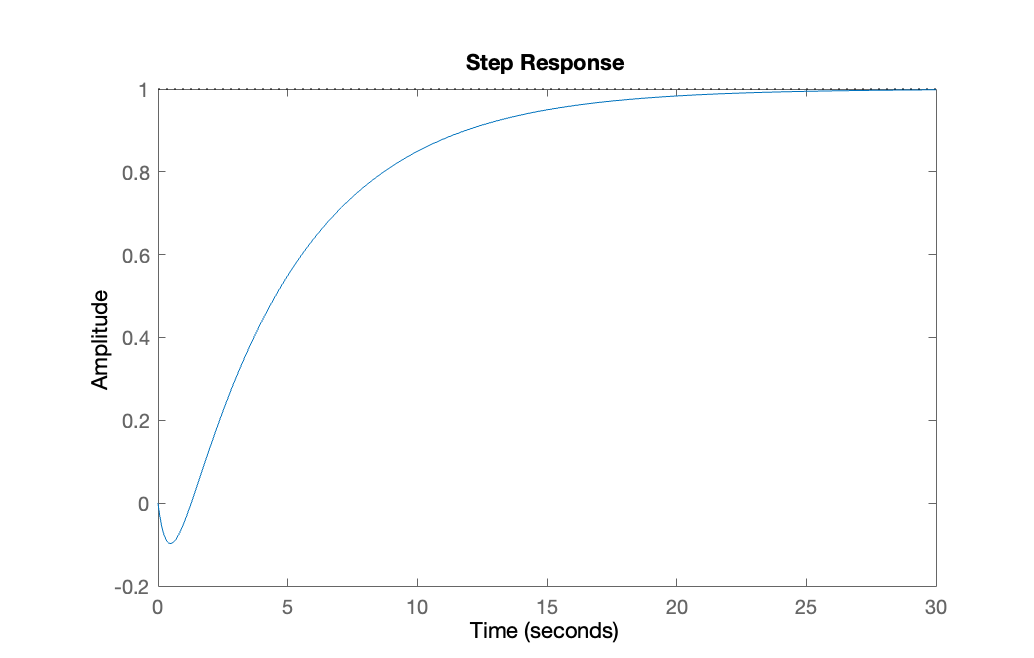
\includegraphics[width=0.8\linewidth]{./figures/Q3_Step_Response.png}
    \caption{Negative Step Response}
\end{figure}

The fact that the response initially moves in the opposite direction of the reference signal is unusual.

\subsubsection*{(d) Create a table of SSE magnitude,
\% undershoot (observed from step response plot)
and settling time (via step response plot)
for K=[0.25,0.45, 0.5, 0.55, 0.75]}

\begin{center}
\begin{tabular}{ |c||r|r|r|r| } 
\hline
    K & SSE Mag & \% Undershoot & Settling Time (s) \\
    \hline
    0.25 & 0.6666 & 15.2627 & 11.0657 \\ 
    0.45 & 0.1818 & 10.7957 & 17.0232 \\ 
    0.50 & 0.0000 & 9.7404 & 19.2101 \\ 
    0.55 & 0.2222 & 8.6896 & 21.8672 \\
    0.75 & 2.0000 & 4.6662 & 42.8983 \\
\hline
\end{tabular}
\end{center}

\subsubsection*{From the results of the table,
what would you say about the sensitivity of this system to K?}

\begin{answer}
\textbf{
From the results of the table, I would say that the system is very sensitive to K.
Any variation of K away from $K = 1/2$ causes the system to incur steady state error.
As K increases, settling time increases greatly. As K decreases, undershoot goes up.
For all three parameters, K has an impact.}
\end{answer}
    
% \color{white}
% \hspace*{6em}\inputminted[frame=leftline,fontsize=\footnotesize]{matlab}
% {./matlab/Problem_5_18.m}
% \color{black}

% \begin{figure}[H]
%     \centering
%     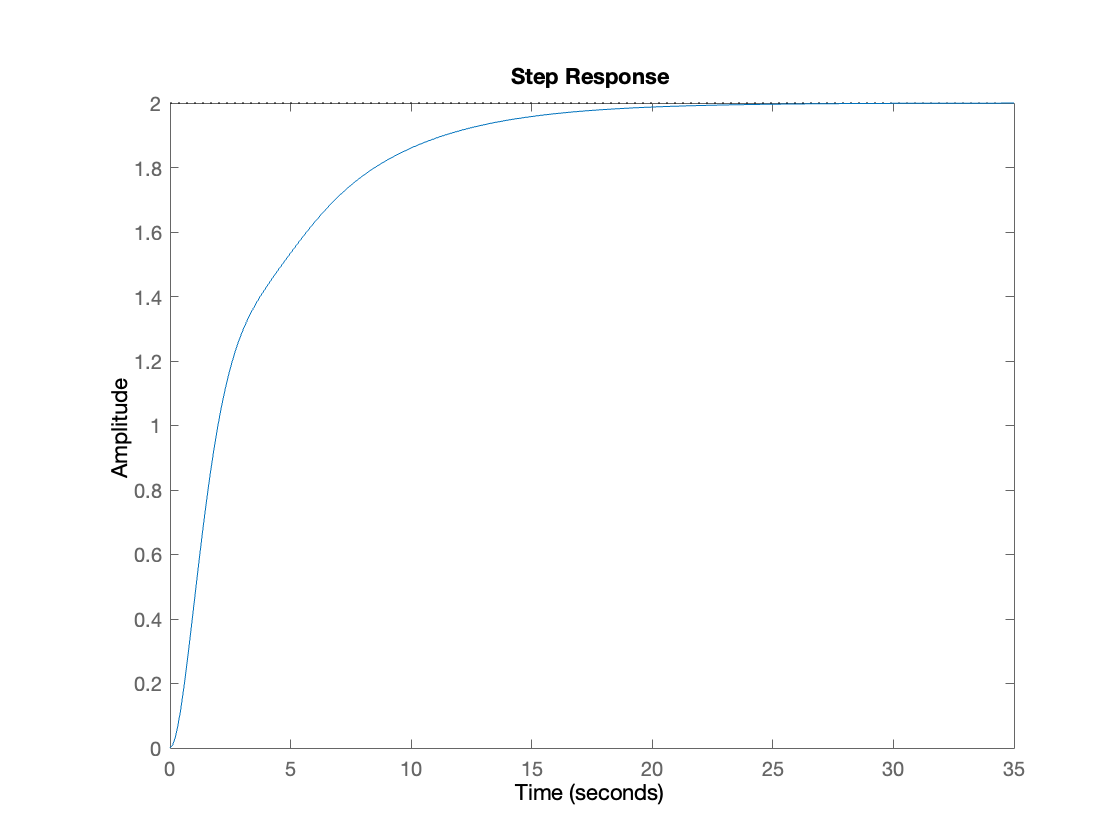
\includegraphics[width=0.7\linewidth]{./figures/step_response.png}
%     \caption{Step Response}
%     \label{fig:step}
%  \end{figure}



\end{document}

